

\chapter{Examining the impact of dynamism on pattern rewriting in static and dynamic languages}
\label{chap:dynamism-pattern-rewriting}


% A key difference between the Python and C++ runtimes is their degree of dynamism.
% \ac{mlir}'s C++ runtime incurs overhead when dynamically dispatching functions (Label \texttt{(3)} of \autoref{fig:narrative}), which is worsened by prohibiting ahead-of-time performance optimisations. In contrast, almost every bytecode operation evaluated by the Python interpreter is dynamic, each incurring an overhead.
% As such, we expect the difference in performance between language runtimes (Label \texttt{(4)} of \autoref{fig:narrative}) to be smaller for more dynamic workloads.
% To corroborate this, we measure the difference in performance between pattern rewriting workloads using xDSL and \ac{mlir}, and assess the contribution of overheads incurred by dynamism.


% Hook
% Argument
% Link





\section{Quantifying the performance impact of dynamism in language runtimes}

% Hook
Dynamism affects performance through a wide variety of mechanisms, in both Python and C++.
% Argument
% Link
In this section, we examine and quantify the impact of some of these mechanisms, substantiating the argument that ...

\subsection{Cost of dynamic dispatch}

% What is dynamic dispatch and how does it work in C++


% How can we measure this?

\begin{figure}[H]
    \centering
    \begin{subfigure}[b]{0.45\textwidth}
       \centering
        \begin{minted}[fontsize=\scriptsize,escapeinside=££]{text}
class Base {
public:
    inline int inlineFunction(int a, int b) {
        return a + b;
    }
    static int staticFunction(int a, int b) {
        return a + b;
    }
    virtual int virtualFunction(int a, int b) {
        return a + b;
    }
    int regularFunction(int a, int b) {
        return a + b;
    }
    virtual ~Base() = default;
};

class Derived : public Base {
public:
    int virtualFunction(int a, int b) override {
        return a + b;
    }
};
        \end{minted}
        \captionsetup{name=Listing}
        \caption{.}
        \label{listing:}
    \end{subfigure}
    \hfill
    \begin{subfigure}[b]{0.5\textwidth}
        \centering
        \begin{minted}[breakanywhere,fontsize=\scriptsize,escapeinside=££]{text}
void go() {
    // Setup
    int a = 5;
    int b = 7;
    int result = 0;
    Base baseObj;
    Derived derivedObj;
    Base* monomorphicPtr = &baseObj;
    Base* polymorphicPtr = &derivedObj;

    // Examples
    result = a + b;
    result = baseObj.inlineFunction(a, b);
    result = Base::staticFunction(a, b);
    result = baseObj.regularFunction(a, b);
    result = baseObj.virtualFunction(a, b);
    result = derivedObj.virtualFunction(a, b);
    result = monomorphicPtr->virtualFunction(a, b);
    result = polymorphicPtr->virtualFunction(a, b);
}
        \end{minted}
        \captionsetup{name=Listing}
        \caption{.}
        \label{listing:}
    \end{subfigure}
    \vspace{1em}
    \captionsetup{name=Listing}
    \caption{.}
    \label{listing:}
\end{figure}

% What are our measurement results? How does this quantify performance in dyunamism?

\begin{table}[H]
  \caption{.}
  \label{tab:dynamic-dispatch-perf}
  \centering
  \begin{tabular}{lllc}
    \toprule
    \multicolumn{3}{c}{\textbf{Function}} \\
    \cmidrule(r){1-3}
    \textbf{Specifier} & \textbf{Morphism} & \textbf{Indirection} & \textbf{Duration [ns]} \\
    % \textbf{Invocation type} & \textbf{Duration [ns]} \\
    \midrule
    Default & Monomorphic & Direct & $0.614$ \\
    Inline & Monomorphic & Direct & $0.614$ \\
    Static & Monomorphic & Direct & $0.613$ \\
    Virtual & Monomorphic & Pointer & $0.613$ \\
    Virtual & Polymorphic & Pointer & $1.07$ \\
    Virtual & Monomorphic & Pointer & $1.98$ \\
    Virtual & Polymorphic & Pointer & $1.90$ \\
    % Function & $0.614$ \\
    % Inline function & $0.614$ \\
    % Static function & $0.613$ \\
    % Monomorphic virtual function & $0.613$ \\
    % Polymorphic virtual function & $1.07$ \\
    % Indirect monomorphic virtual function & $1.98$ \\
    % Indirect polymorphic virtual function & $1.9$ \\
    \bottomrule
  \end{tabular}
\end{table}



\subsection{Dynamism hiding ahead-of-time optimisations}



\subsection{Runtime type information}

%% C++ RTTI vs LLVM RTTI

%% Python RTTI

% How can we measure this?


% What are our measurement results? How does this quantify performance in dyunamism?






% \subsection{Specialised and unspecialised instructions}

% % Hook
% As discussed in \autoref{sec:specialising-adaptive-interpreter}, Python's specialising adaptive interpreter
% % Argument
% % Link
% In contrast to the previous examples where introducing more dynamism hinders performance, this is an example of where removing dynamism can result in performance improvements.

% % Specialist something something.....






\section{Dynamism in xDSL}

% Hook
% Argument
% Link

\subsection{Operation trait checks}

% Hook
Having specialised xDSL's \mintinline{python}{has_trait} method to the most minimal implementation which expresses the desired functionality, we can draw comparisons between equivalent algorithms which predominantly measure the effect of the language runtime.
% Argument
Both implementations (Listing \ref{listing:ubenchmark-trait-checks-both}) share the same underlying algorithm: iteration over an operations traits, checking against each one. However, the mechanism used for this algorithm differs significantly between xDSL and MLIR.
By leveraging Python's dynamic nature, xDSL can invoke the \mintinline{python}{isinstance} function to check each trait. In contrast, MLIR uses template metaprogramming instead of the class hierarchy to define traits. This depends on \mintinline{c++}{TypeID}\footnote{\url{https://mlir.llvm.org/doxygen/TypeID_8h_source.html}}, a custom data structure to encode dynamic \ac{rtti} in C++.
% TODO: Does this need more detail?
Whilst this implementation incurs complexity (\autoref{fig:ubenchmark-hastrait-dynamism}), it remains performant, as the \mintinline{c++}{TypeID} data structure is constructed to remedy many of the issues of native C++ \ac{rtti}.
% Link
However, this dynamism impacts performance beyond just the runtime of the individual function, as it presents an optimisation boundary -- precluding other optimisations which could be applied if the result could be inferred at compile time. % TODO: This really needs to be substantiated somehow, but perhaps not here?

\begin{figure}[H]
    \centering
    \begin{subfigure}[b]{\textwidth}
        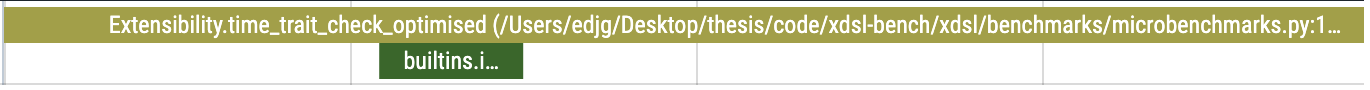
\includegraphics[width=\textwidth]{images/impact_dynamism/hastrait_xdsl_viztracer_optimised.png}
        \caption{\texttt{viztracer} trace of xDSL's optimised \mintinline{python}{has_trait} implementation.}
        \label{fig:ubenchmark-hastrait-xdsl-viztracer-optimised}
    \end{subfigure}
    \begin{subfigure}[b]{\textwidth}
        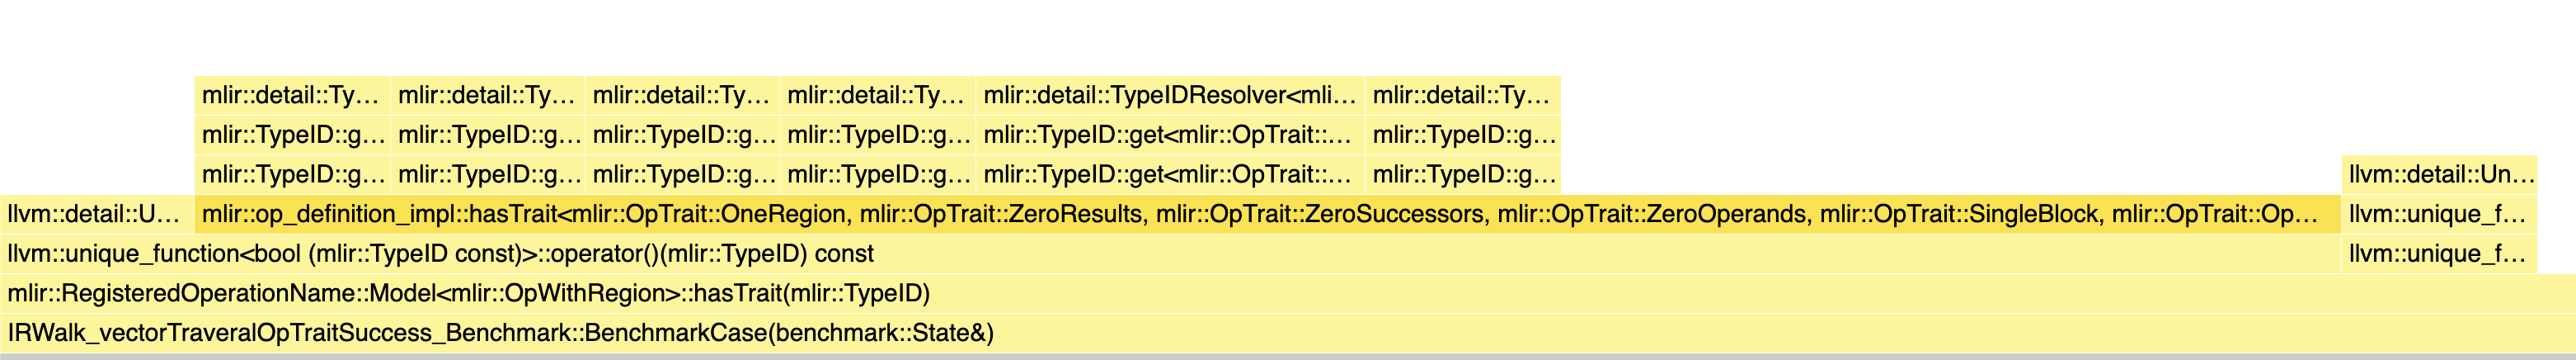
\includegraphics[width=\textwidth]{images/impact_dynamism/hastrait_mlir_samply.png}
        \caption{\texttt{samply} trace of MLIR's \mintinline{c++}{has_trait} method.}
        \label{fig:ubenchmark-hastrait-mlir-samply}
    \end{subfigure}
    \caption{MLIR's dynamic trait checking using C++ RTTI is more complex than xDSL's Python implementation using \mintinline{python}{isinstance}.}
    \label{fig:ubenchmark-hastrait-dynamism}
\end{figure}


% \subsection{Constant folding}

% Hook
% Argument
% Link

% Hook
% Argument
% Link

% Hook
% Argument
% Link


\section{Summary}

% Hook
% Argument
% Link

% Hook
% Argument
% Link
